\chapter{Технологическая часть}

В данном разделе производится выбор средств реализации, а также приводятся листинги реализованных алгоритмов и результаты тестирования программы.


\section{Выбор средств реализации}

Основное требование к языку программирования в данной лабораторной работе - наличие в нем нативных потоков. Язык C++ обладает этим свойством и уже использовался мною ранее, поэтому и был выбран  \cite{CBook}. 

Для замеров времени используется предоставляемый класс system\_clock::time\_poin, использующий данные системных часов в реальном времени \cite{CBook2}, а для организации распараллеливания -  std::thread.

В качестве среды разработки выбран “QT Creator” так как она была часто использована мною ранее.


\section{Реализация алгоритмов}

\lstset{style=с++}

В листингах \ref{tras_basic} - \ref{tras_work} представлены реализации рассматриваемых алгоритмов.

\begin{lstlisting}[caption=Реализация  последовательного алгоритма трассировки лучей,
	label={tras_basic}]
public Bitmap render_simple()
{
	Camera camera = scene.camera;
	Vec3 view_vector = null;
	Vec3 color = null;
	for (int x = -scene.canvasWidth / 2; x < scene.canvasWidth / 2; x++)
	{
		for (int y = -scene.canvasHeight / 2; y < scene.canvasHeight / 2; y++)
		{
			view_vector = ProjectPixel(x, y) * camera.rotation_mtrx;
			color = TraceRay(camera.position, view_vector, projection_plane_d, Double.PositiveInfinity, recursion_depth, x, y);
			SetPixel(x, y, CountColor(color));
			
		}
	}
	
	return this.bmp;
}
\end{lstlisting}


\begin{lstlisting}[caption=Реализация главного потока параллельного алгоритма трассировки лучей,
	label={tras_main}]
public Bitmap render_parallelized()
	{
		Thread[] threads = new Thread[numThreads];
		for (int i = 0; i < numThreads; i++)
		{
			Limits p = new Limits(scene.canvasWidth / numThreads, scene.canvasHeight, -scene.canvasWidth / 2 + scene.canvasWidth / numThreads * i, -scene.canvasHeight / 2);
			threads[i] = new Thread(render_par_working);
			threads[i].Start(p);
		}
		foreach (Thread thread in threads)
		{
			thread.Join();
		}
		
		return this.bmp;
	}
\end{lstlisting}

\begin{lstlisting}[caption=Реализация рабочего потока параллельного алгоритма трассировки лучей,
	label={tras_work}]

	public void render_par_working(object obj)
	{
		Limits p = (Limits)obj;
		Camera camera = scene.camera;
		Vec3 view_vector = null;
		Vec3 color = null;
		for (int x = p.start_x; x < p.start_x + p.width; x++)
		{
			for (int y = p.start_y; y < p.start_y + p.height; y++)
			{
				view_vector = ProjectPixel(x, y) * camera.rotation_mtrx;
				color = TraceRay(camera.position, view_vector, projection_plane_d, Double.PositiveInfinity, recursion_depth, x, y);
				SetPixel(x, y, CountColor(color));
				
			}
		}
\end{lstlisting}

\section{Тестирование}

На рисунке \ref{fig:work_example} приведен результат тестирования программы по методу черного ящика: проведен запуск программного обеспечения для рендера сцены, состоящей из поверхности земли, повехности неба (стена на некотором расстоянии с текстурой) и флюгера (сложносоставной модели), добавлены два источника света -- один точечный и один направленный. Программа успешно выполнила рендер сцены на восьми потоках, изображение совпало с ожидаемым -- с тем, которое было получено при запуске последовательной версии алгоритма. На рис. \ref{fig:work_example} представлено полученное изображение.

\newpage
\begin{figure}[h!]
	
	\centering{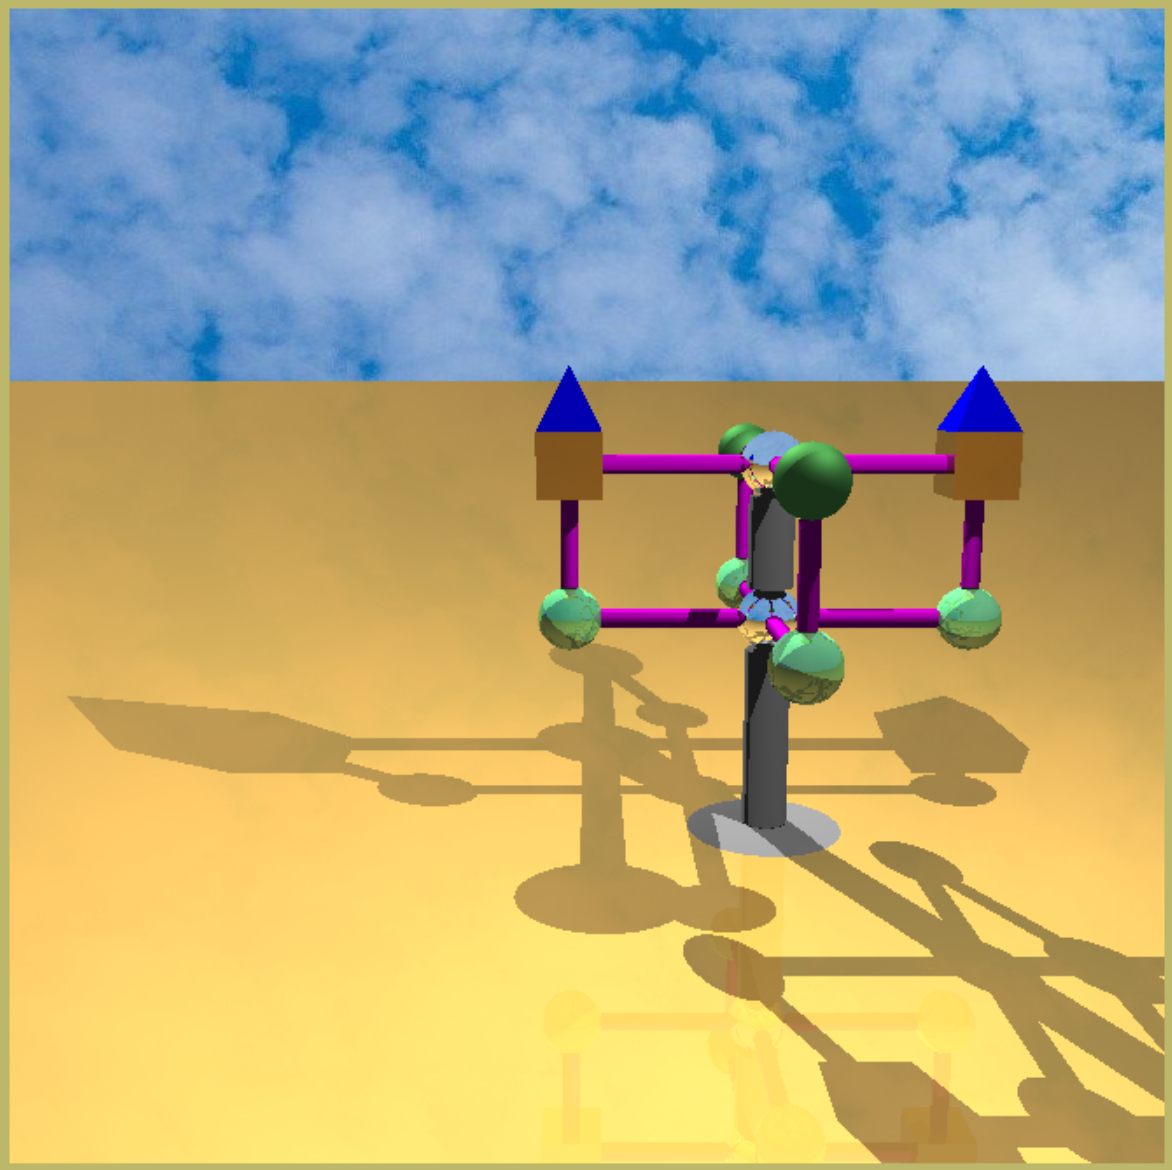
\includegraphics[scale=0.7]{inc/img/work_example.png}}
	
	\caption{Результат тестирования программы}
	
	\label{fig:work_example}
	
\end{figure}


\section{Вывод из технологической части}

Был производен выбор средств реализации, реализованы и протестированы последовательный и параллельный алгоритмы обратной трассировки лучей.
